\subsection{Standardizing start times}
Most pain scores in the data file begin shortly after surgery, with about 80\% starting within two hours post-operation. However, there is a non-trivial subset of patients whose pain score recordings started up to several days after their surgeries, as shown in Figure \ref{fig:start_times}.

\begin{figure}[h]
        \begin{subfigure}{0.5\textwidth}
                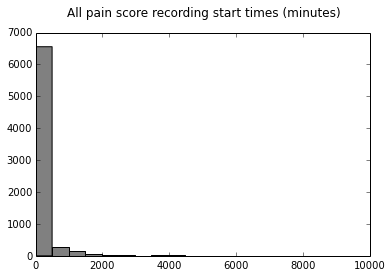
\includegraphics[width=\textwidth]{Figures/pain_score_start_times.png}
                \caption{Normal scale}
                \label{fig:start_times_normal}
        \end{subfigure}\begin{subfigure}{0.5\textwidth}
                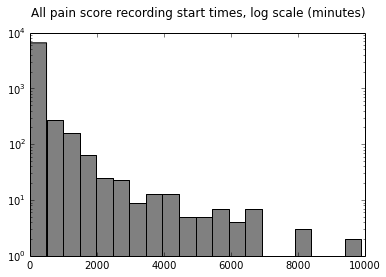
\includegraphics[width=\textwidth]{Figures/pain_score_start_times_log.png}
                \caption{Log scale}
                \label{fig:start_times_log}
        \end{subfigure}
        \caption{Histograms of all pain score start times in minutes, both normal and logarithmic scales}\label{fig:start_times}
\end{figure}

In the interest of analyzing pain profiles along a standard post-operation time interval, data was disregarded for those patients whose pain scores were recorded starting more than two hours after their procedure. This operation retained 80\% of the original data set. Figure \ref{fig:start_times_pruned} shows the set of start times less than two hours post-operation.

\begin{figure}[h]
        \begin{subfigure}{0.5\textwidth}
                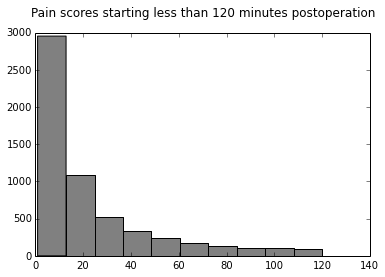
\includegraphics[width=\textwidth]{Figures/pain_score_start_times_lte2hours.png}
                \caption{Normal scale}
                \label{fig:start_times_pruned_normal}
        \end{subfigure}\begin{subfigure}{0.5\textwidth}
                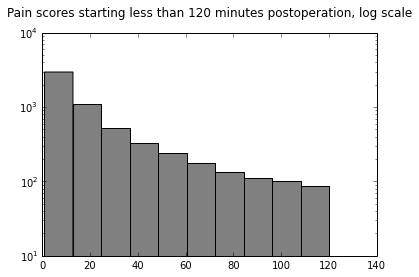
\includegraphics[width=\textwidth]{Figures/pain_score_start_times_lte2hours_log.png}
                \caption{Log scale}
                \label{fig:start_times_pruned_log}
        \end{subfigure}
        \caption{Histograms of all pain score start times less than 120 minutes, both normal and logarithmic scales}\label{fig:start_times_pruned}
\end{figure} 